%%%%%%%%%%%%%%%%%%%%%%%%%%%%%%%%%%%%%%%%%%%%%%%%%%%%%%%%%%%%%%%%%%%%%%%
%% Einleitung
\section{Einleitung}
\label{sec:einleitung}

Der Demographische Wandel in Deutschland stellt die Gesellschaft und die Politik vor ein großes Problem. Nicht nur der fehlende Nachwuchs, der ein Arbeitnehmerloch hinterlässt, sondern auch eine immer älter werdende Gesellschaft sorgen für viele Fragezeichen. Neben kommunalen Problemen, wie teure Infrastruktur, ist eins der größten Anliegen die Altersarmut. Ein sinkendes Rentenniveau und steigende Kosten werden es in Zukunft unmöglich machen für eine gute Pflegeversorgung zu bezahlen. \citep{brunozandonella2013} Neben den hohen Kosten in der Pflege sind auch andere Faktoren die zu einer nicht akzeptablen Situation führen. So ist der Pflegeberuf zu unattraktiv für viele junge Menschen, wodurch auch hier ein großes Loch an Arbeitnehmern\FemaleMale wahrzunehmen ist. Körperlich anstrengende Arbeit, die in kurzer Zeit ausgeführt werden muss, führen zu vielen physischen und psychischen Erkrankungen der Pfleger\FemaleMale .\citep{AOK2004}

Einen alternativen Weg bringt die Technik. Einfache zu bedienende Systeme können den Alltag vereinfachen und so auch älteren Menschen ein selbstständiges Leben ermöglichen. Alltägliche Aufgaben müssten nicht mehr von Pflegern\FemaleMale übernommen werden, sondern könnten durch Maschinen erledigt werden. Schon heute können einzelne Kleinsysteme Haustätigkeiten wie Staubsaugen und Rasenmähen übernehmen. Ein Vorreiter auf diesem Gebiet ist das Roboterland Japan. Dort überlegte Kobayashi Hisato, Professor für Maschinenbau und Robotik an der Hosei-Universität in Tokio, sich schon 1999 Konzepte für Senioren-Service Roboter.\citep{wagner2009tele}  Nach seinen Vorstellungen sollten dabei Roboter nicht autonom arbeiten, sondern von Familienangehörigen ferngesteuert und überwacht.\citep{kobayashihisato1999} Neben diesen Konzepten kann man aber auch schon angewandte Robotik in Japans Seniorenpolitik finden. Zwei Musterbeispiele zeigen dabei die unterschiedlichen Anwendungsszenarien für Roboter im privaten Umfeld. \textit{Sinére K\={o}rien} der Firma Matsushita ist ein digitales Seniorenheim. Neben einer Smarthouse Anbindung gehört auch der Roboterteddy K\={o}-chan zur Ausstattung der einzelnen Zimmer. Dieser dient als Unterhaltungsroboter und Kommunikationsgerät mit den Pflegern\FemaleMale. So kann mit den Kameraaugen im Teddy eine Aufnahme vom Raum gemacht werden und im Notfall den Pflegern\FemaleMale eine Alarmmeldung geschickt werden. Weitere Sensoren, zu  Beispiel Gewichtssensoren unter den Betten, geben Informationen über die Abwesenheiten von Patienten\FemaleMale.\citep{wagner2009tele} Ein weiterer Anwendungsbereich für Roboter ist die \textit{robotto serap\={\i}} (Robotertherapie). Dabei beschäftigen sich die Senioren\FemaleMale mit tierähnlichen Robotern, wie Hunden, Seeroben oder Katzen. Im Zentrum der Therapie steht die Interaktion zwischen Patient\FemaleMale und Roboter. Die Robotertherapie soll die Patienten\FemaleMale aktivieren und deren Tagesabläufe abwechslungsreich gestalten. Außerdem steigert es die Kommunikation zwischen zwei Patienten\FemaleMale, die am selben Roboter arbeiten. \citep{wagner2009tele}

 \begin{figure}
 	\centering
 	\subfigure[Roboterteddy K\={o}-chan Quelle: \citep{panasonic2005}]{%
 		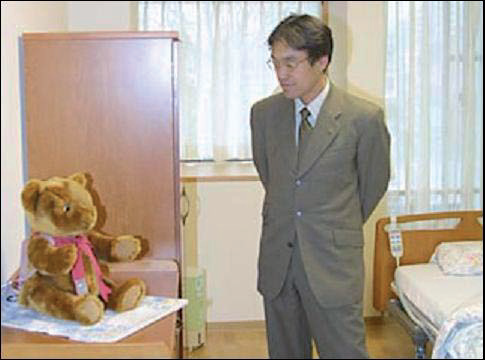
\includegraphics[scale=0.6]{fig/roboteddy}
 		\label{fig:roboTeddy}}
 	\hfill
 	\subfigure[Roboterkatze zur Therapie Quelle: \citep{wagner2009tele}]{%
 		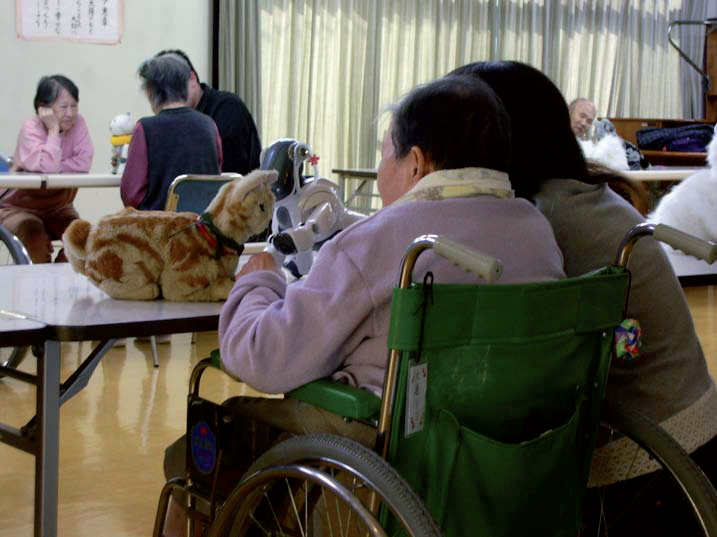
\includegraphics[scale=0.4]{fig/robocat}
 		\label{fig:roboTeddy2}}
 	\caption{Roboter in Seniorenheimen}
 	\label{fig:robSenioren}
 \end{figure}

Nicht nur in Japan, sondern auch in Deutschland wird sich mit dem Thema \textit{Care(rob)bots} befasst. So finden sich unter dem Stichpunkt \textit{Mensch-Maschine-Entgrenzungen} Studien zu der Thematik. Andere Untersuchungen befassen sich mit der Gegenseite, der Akzeptanz der Senioren\FemaleMale für Roboter. So ergab eine Befragung der VDE-Studie "Mein Freund der Roboter", dass eine Mehrheit (56\%) der Senioren\FemaleMale Robotern im Haushalt offen gegenüber stehen und diese einem Pflege-/Altersheim vorziehen würden. Neben den bekannten Staubsauger- und Rasenmährobotern, sind es auch zukünftige Anwendung, wie ein roboterisierter Rollstuhl, die hohe Akzeptanzwerte erreichen. Die Studie zeigte aber auch, dass Senioren\FemaleMale zunächst Robotern skeptisch gegenüberstehen. Spontan lehnten 40 Prozent der Senioren\FemaleMale Roboter in ihrem privaten Umfeld ab, 60 Prozent empfanden Robotik sogar als unheimlich. jedoch zeigte sich, dass der Wunsch nach einer selbstständigen Lebensführung ein starker Faktor für die Akzeptanz ist. Dadurch ergibt sich eine Beliebtheit für Serviceroboter. So sind Roboter, die abgrenzbare Tätigkeiten im Haushalt selbständig erledigen, sehr beliebt. Wichtige Kriterien für die Akzeptanz waren zudem die intuitive Bedienbarkeit, die Robustheit und die Flexibilität gegenüber unterschiedlicher Handicaps. Auch menschliche Faktoren wie Geduld, Verständnis, Höflichkeit und Achtung der Intimsphäre waren den Anwendern\FemaleMale wichtig.\citep{dr.sibyllemeyer2011}

Neben den sozialen Forschungen gibt es in Deutschland auch ingenieurwissenschaftliche Ergebnisse auf diesem Gebiet. So beschäftigt sich das  Cluster of Excellence Cognitive Interaction Technology (CITEC) in Bielefeld, zusammen mit der Stiftung Bethel, in der Forschung auf dem Gebiet der Unterstützung für Demenzkranke. Die dort entwickelten Assistenzsysteme helfen den Patienten unter anderem beim Zähneputzen und geben ihnen so ein Stück Selbstständigkeit zurück.

Viele Forschungen und Entwicklungen beschäftigen sich momentan mit der Mensch-Maschine/Roboter Beziehung. Dabei geraten die Roboter-Roboter-Interaktionen in den Hintergrund. Da aber heutige Roboter keine Allround-Lösungen bieten, sondern meist hochgradig spezialisiert sind und nur eine Tätigkeit ausführen können( zum Beispiel Saugroboter, Fensterwischroboter und weitere), ist das Zusammenspiel und die Komposition der Roboter wichtig. Das Szenario in Abbildung \ref{fig:szen1} zeigt, wie solch eine Komposition aussehen könnte.

\begin{figure}
	\centering
	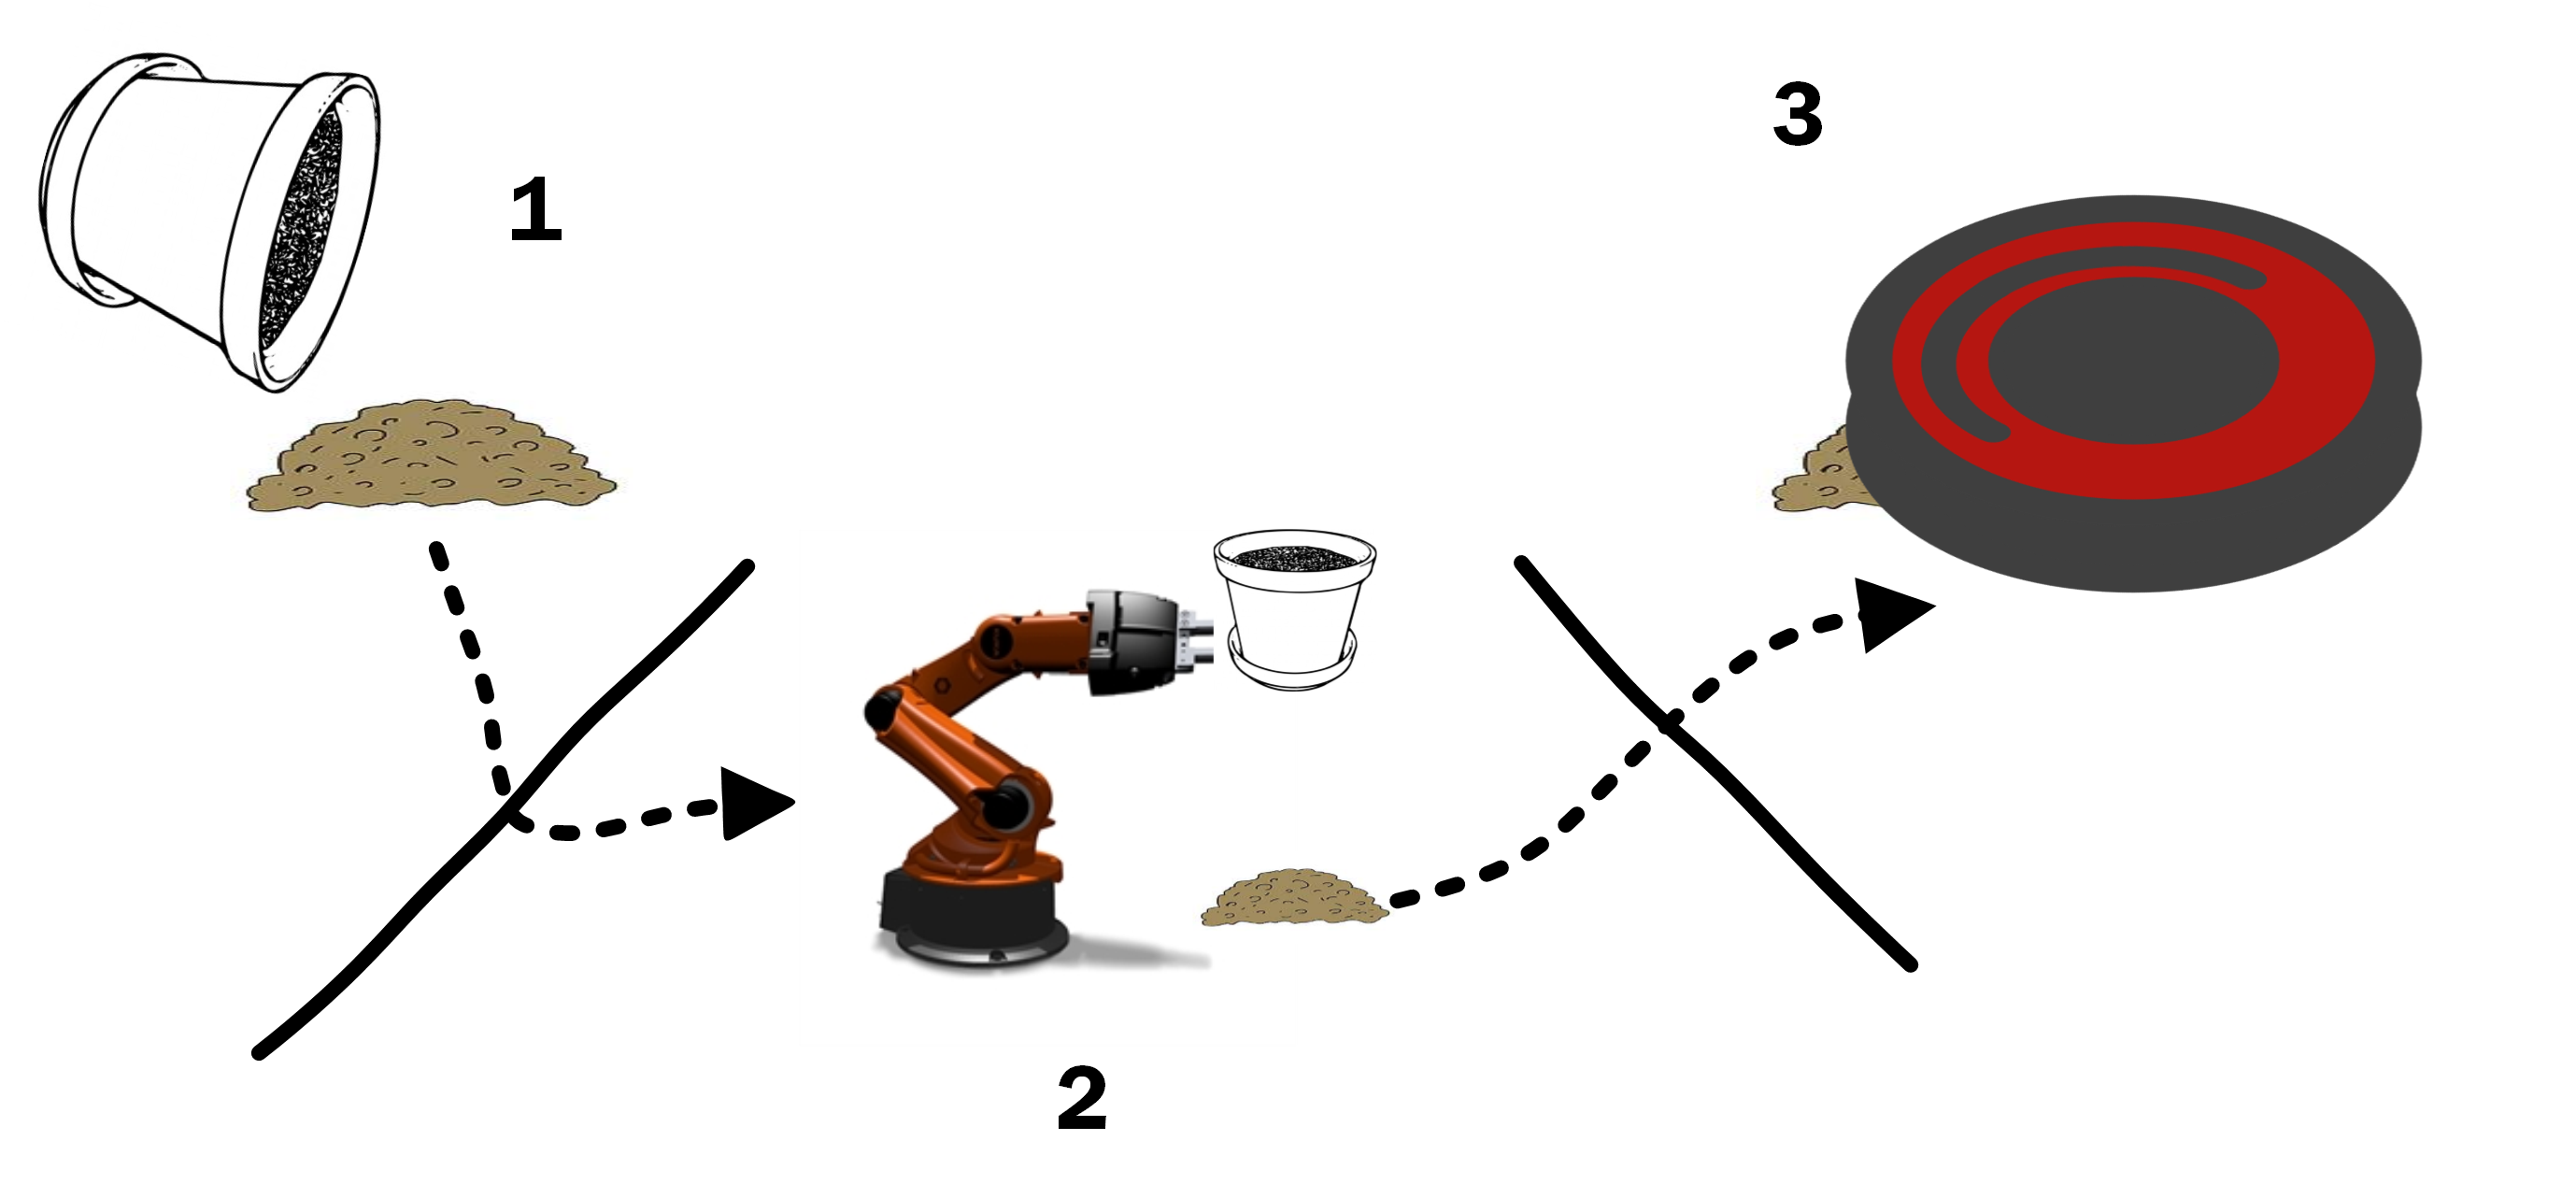
\includegraphics[scale=1.4]{fig/szen1}   
	\caption[Beispiel Szenario 1]{Mensch A stößt einen Blumentopf um (1). Ein Kamerasystem dediziert das der Topf umgefallen ist und Erde auf dem Boden liegt. Ein Roboter mit Arm wird gerufen, der zunächst die Vase aufhebt und an ihren Platz zurückstellt (2). Anschließend wird ein Saugroboter aktiviert, der die Erde weg saugt (3). Bei schwereren Verschmutzungen wird noch ein Wischroboter bestellt.}
	\label{fig:szen1}
\end{figure}

Dabei führt jeder Roboter selbstständig  und unabhängig von den anderen seine Arbeit aus. Die Kommunikation geht immer von der Zentralen Steuereinheit, dem \textit{Master}, aus. Zwischen den einzelnen Robotern findet kein großer Informationsaustausch statt. Die Änderung an dem Szenario in Abbildung \ref{fig:szen2} ändert jedoch die Art der Zusammenarbeit und der Kommunikation. Nun ist es nötig, dass die Roboter notwendige Informationen, wie die Übergabepose oder eine Synchronisierung der Gripper, austauschen.

\begin{figure}
	\centering
	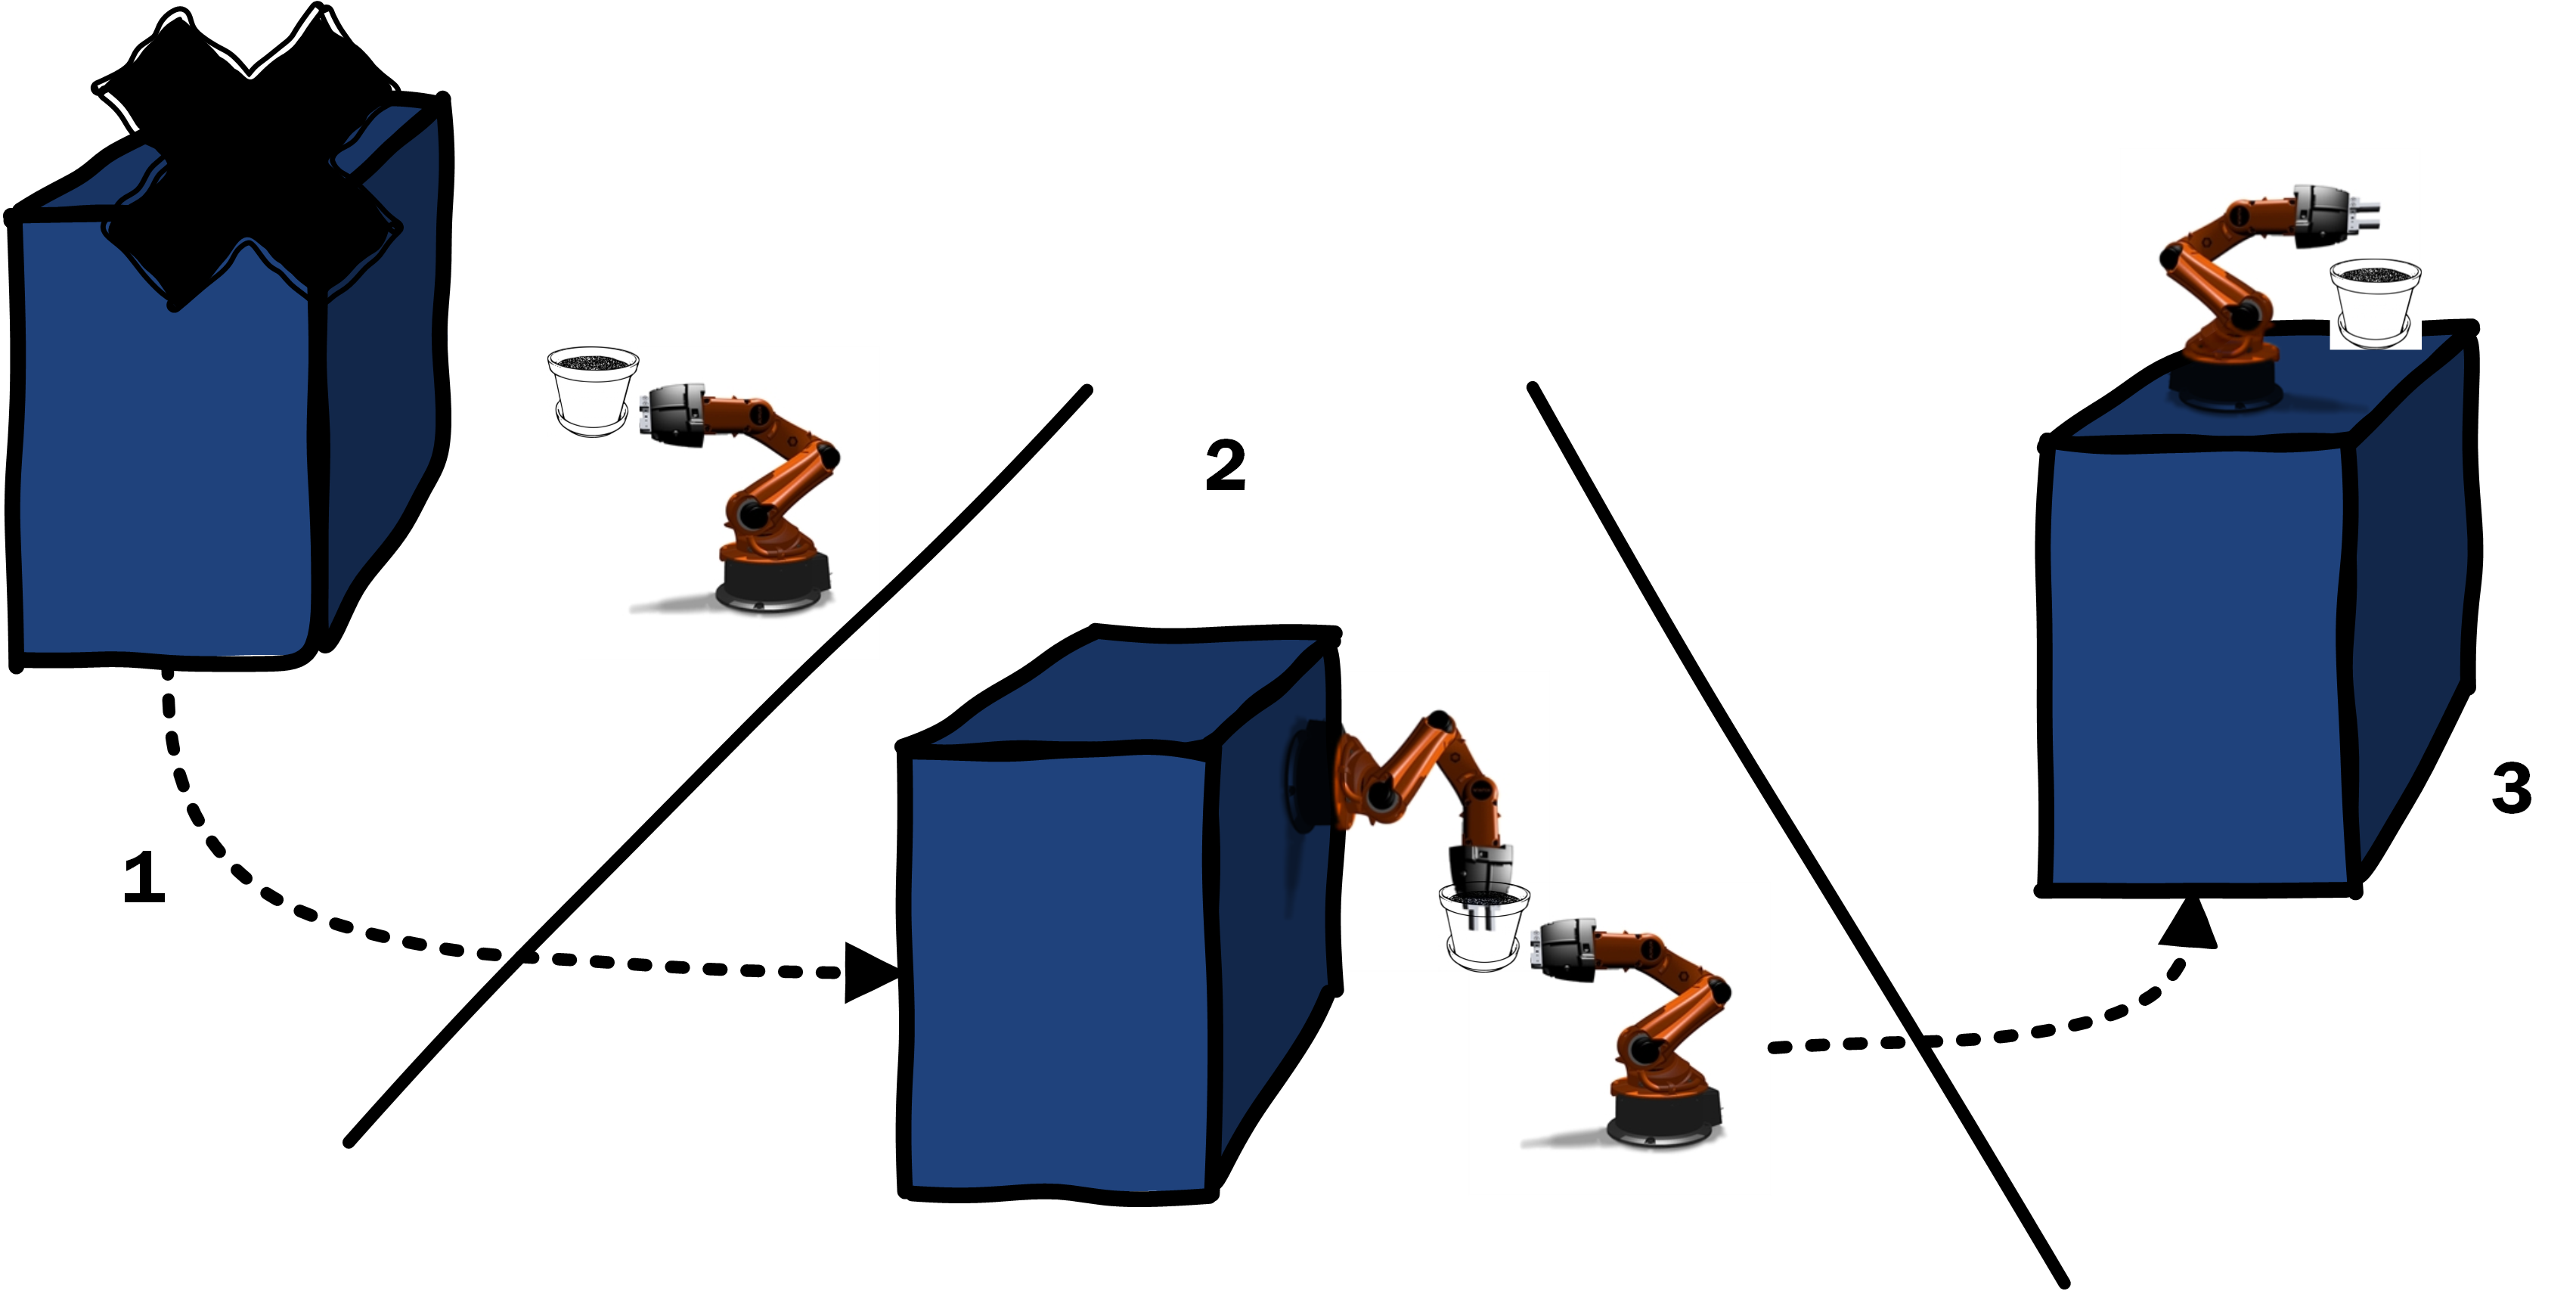
\includegraphics[scale=1.0]{fig/szen2}   
	\caption[Erweiterung Szenario 1]{Beim Zurückstellen der Vase stellt der Roboter fest, dass er die gewünschte Position nicht erreichen kann(1), weil sein Arm zu kurz ist. Da auf der Anrichte noch ein weiterer Arm steht nimmt er die Kommunikation mit diesem Manipulator auf. Sie kommunizieren einen Übergabepunkt und führen ein Übergabemanöver durch. Arm 2 stellt nun die Vase an die gewünschte Position.
	}
	\label{fig:szen2}
\end{figure}


Der zentrale Aspekt dieser Arbeit befasst sich mit der Abstraktion von Szenario 2. Roboter 1 übergibt ein Objekt an Roboter 2. Dabei werden verschiedene Thematiken aufgegriffen, untersucht und erläutert. Das Folgende Kapitel befasst sich mit den Grundlagen dieser Arbeit, es werden einzelne Begriffe aus der Robotik und der Middleware \textbf{R}obot \textbf{O}perating \textbf{S}ystem erläutert, sowie der genutzte Laboraufbau dargestellt. Dabei wird die verwendete Hardware aufgelistet und im Detail betrachtet. Kapitel \ref{sec:relatedwork} zeigt schon bestehende Arbeiten im Bereich Robotik, die mit dieser Arbeit in Zusammenhang bestehen. So wird unter anderem der Begriff PEIS (Physically Embedded Intelligent Systems) erläutert und die Verbindung zur Thesis gezeigt. Des Weiteren werden Arbeiten für Multirobot Systeme und Handover-Methoden erklärt. Im darauf folgenden Kapitel 




